\section{Modulo Servicios Turísticos}

\subsection{Objetivo}
El objetivo de este módulo es poder gestionar los servicios turísticos pertenecientes a una zona y asociarles un nombre, puntuación, descripción, ubicación geográfica e imagenes.

\subsection{Diseño}

Una zona turística consta de múltiples servicios turísticos los cuales están identificados geográficamente por coordenadas, permitiendo a la aplicación móvil identificarlos y generar una ruta eficaz.


\subsection{Desarrollo}

Los servicios turísticos se marcan al igual que las zonas a través de una API implementada por Mapbox, las geocercas se delimitan gráficamente y el sistema obtiene las coordenadas para depositarlas en un JSON donde serán consumidas por el módulo móvil.

\subsection{Resultados}

La Figura \ref{fig:servicios} muestra la pantalla principal donde se enlistan y gestionan  los servicios turísticos pertenecientes a una zona, así mismo en la figura \ref{fig:agregarserv} se observa la pantalla correspondiente al ingreso de la información de un servicio.\\

\begin{figure}[htbp]
	\begin{center}
		\fbox{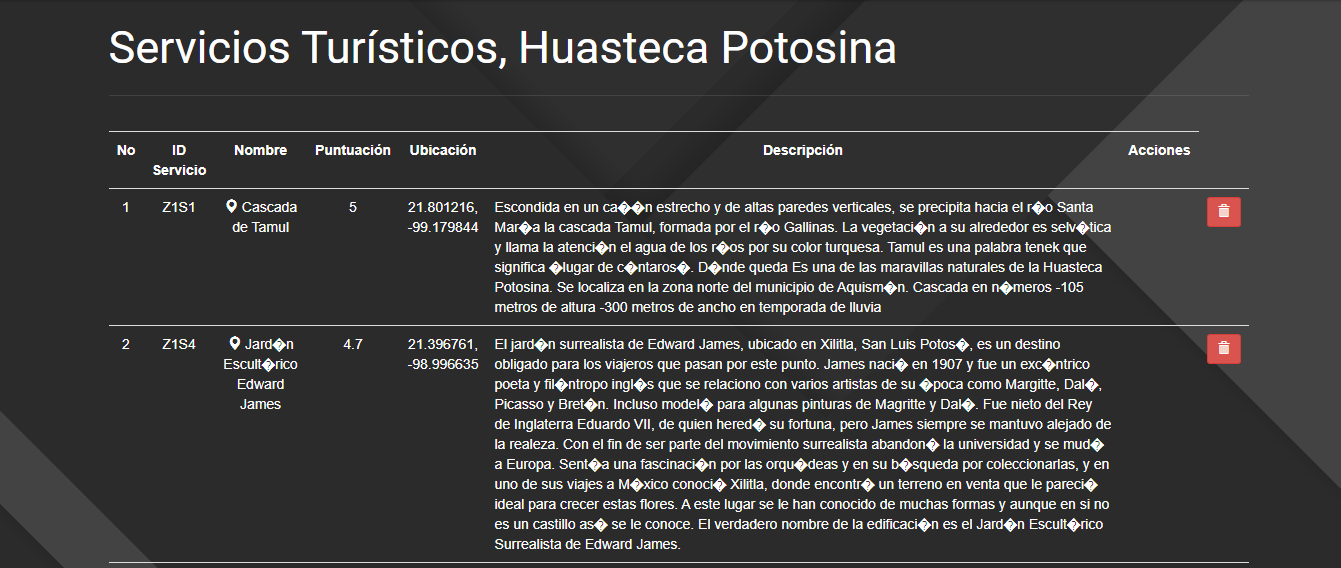
\includegraphics[scale = .6]{implementacion/servicios/images/servicios}}
		\caption{Gestón de Servicios Turísticos}
		\label{fig:servicios}
	\end{center}
\end{figure}

\begin{figure}[htbp]
	\begin{center}
		\fbox{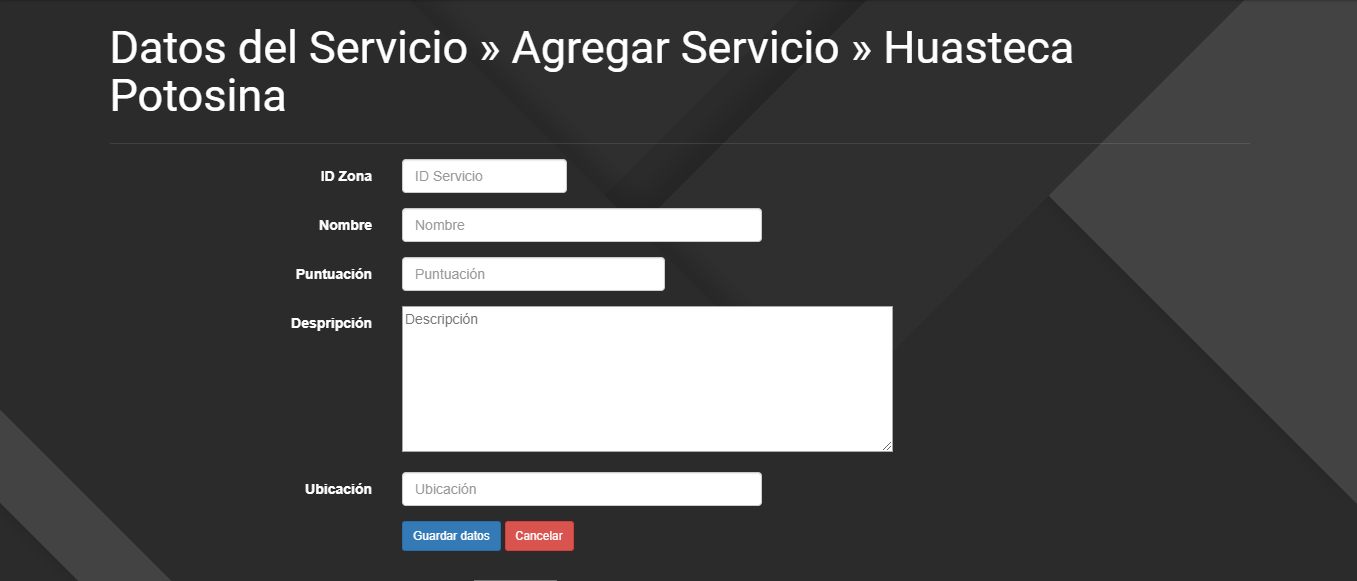
\includegraphics[scale = .6]{implementacion/servicios/images/agregar}}
		\fbox{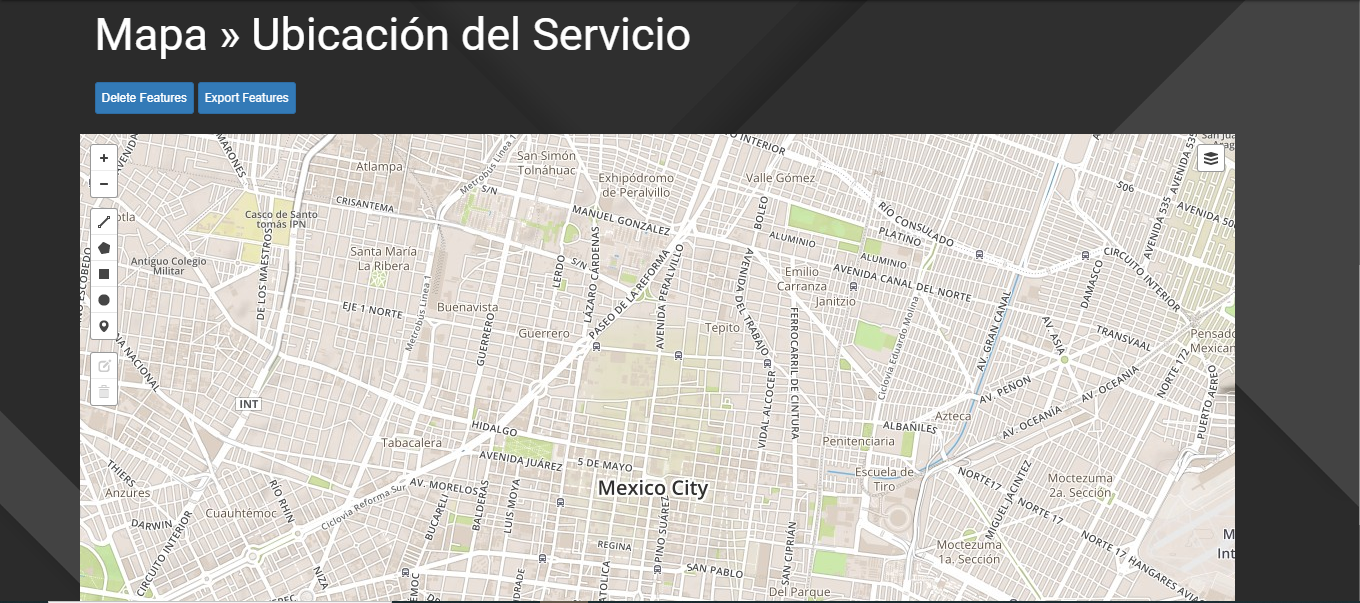
\includegraphics[scale = .5]{implementacion/servicios/images/mapa}}
		\caption{Agregar Servicio Turístico}
		\label{fig:agregarserv}
	\end{center}
\end{figure}



